\chapter[The End - Ideas and Final Remarks]{The End - Ideas and Final Remarks}\label{chap:the_end}
% LINGO: unorthodox.
In the last chapter of this thesis, I would like to present some ideas for future research in persuasive password support. Although I would have loved to start working on these already now, they go beyond the scope of this thesis and should be left to future work. As final remarks, I want to share my views on current developments of password authentication, where I see it in the near future, and how its future can be shaped more positively. 

\section{Ideas for Future Work}
The recommendations in Section \ref{sec:summary:recommendations} touched on future work on a high level. However, one recommendation was to follow up on ideas off the beaten path. Addressing this criterion, the following sections provide more specific ideas to work on password support in the future. 

%-- be frank and say we don't want to create ``recommendations'' or ``guidelines'', because it takes years and more diverse samples to solidify such. Therefore, we think it's better to show ``ideas'' what this can mean and where the topic is going. 

%TODO keep in mind: relate all ideas to the P4P framework. 
\subsection{Follow-Up Studies} 
% combine PASDJO and Personality study.
First and foremost, it will be worthwhile to address the limitations of the studies we conducted, or follow up on the leads from initial results. For instance, the PASDJO deployment in the wild suffered from lack of demographic data to understand individual differences in password perception. The second study on personality lacked more randomness of the available passwords and it would thus be straightforward solution to integrate a short, optional psychometric questionnaire into PASDJO. Alternatively, we could have crowd-workers fill out a more elaborate psychometric survey before they play PASDJO and then fit regression models on the data. In any case, by combining the two approaches we will overcome current limitations of the two studies at once. 

% of course the password reuse manager. 
Furthermore, it will be vital to evaluate the Password Reuse Manager (PWRM, see Chapter \ref{chap:perdespassup}) with a longitudinal study. At this point, we used a rapid iterative design method that was focused on qualitative feedback on features. The next step will be to invite a larger audience to test it for at least one month. To boost usage numbers during the field trial, the browser extension can be made compatible with additional browsers with very little effort. It is already built on the WebExtensions API, which is increasingly solid on all major browsers. We had also identified specific research questions that can be answered with A/B testing. One of the issues was that users kept their previous password managers activated and the additional extension simply generated more effort. The follow-up study should therefore screen for participants who do not use a password manager yet (group A), and another group who will be required to move over to the PWRM as single management solution throughout the entire study (group B). To extend the method space (see recommendation \ref{recommendation:method_space} in Section \ref{sec:summary:recommendations}) and better understand how the support works for the users, the study should conclude with the \textit{break up-/love-letter method}\footurl{https://medialabamsterdam.com/toolkit/method-card/break-uplove-letter/}{28.03.2018}. Here, participants decide whether to write a love or a break-up letter to the PWRM, which will allow us to understand the emotional component of password support. 

% in-situ
Finally, some of our other studies involved a password \textit{creation} task (see Chapters \ref{chap:pws_and_personality},\ref{chap:decoy}, and \ref{chap:emojipasswords}). Although we followed guidelines to establish realistic scenarios, we would have been desirable to study password selection in-situ. Thus, in the future, we should leverage existing web-applications to test concepts when they are mature enough. Establishing collaborations with industry partners is critical to carry out this research approach. 

\subsection{Personalizing Password Policies}\label{sec:pst:personalizing-policies}
Personalization is a current big trend in user experience design and persuasive technology\footurl{https://www.forbes.com/sites/shephyken/2017/05/13/recommended-just-for-you-the-power-of-personalization/}{28.03.2018}, especially since the breakthrough in machine-learning capabilities. It was already an element in the Persuasive Authentication Framework \cite{Forget2007PersuasionEducationSecurity}. We have found that personality has a notable influence on how users perceive password policies (see Chapter \ref{chap:pws_and_personality}). Therefore, it is conceivable to leverage state-of-the-art computing power to tailor password requirements to individual users instead of relying on a one-fits-all approach. Hypothetically, if the system could detect what policy will \textit{help} the user to find the best trade-off between password strength and usability the user experience of using the system would not be degraded by password authentication (as it is now). I provided initial pointers about the benefits in a position paper adjunct to \textit{PERSUASIVE'17} \cite{Seitz2017PersonalizingPasswordPolicies}. 

Tackling this challenge is possible with several focus areas, where the P4P framework can guide design decisions. For instance, we could advance algorithms to detect re-used passwords more reliably at registration. Khern-am-nuai \etal have showed an initial proof-of-concept that keystroke dynamics provide useful features \cite{Khern-am-nuai2017Journal}, but the analysis was done post-hoc. Machine-learning can potentially enable reuse detection already at enrollment and allow us to tailor feedback more appropriately. For instance, we can design a solution that makes alternatives to password reuse more salient, in case reuse generates considerable risks (process depicted in Figure \ref{fig:summary:flow-chart}). Similar approaches are conceivable with different personality profiles. However, here it is much more likely to tailor personalize support strategies during password \textit{reset}, because the service potentially possesses more data about the user at that point. 
%TODO: argumentation ist noch nicht ganz geradlinig. 

\begin{figure}[htbp]
	\centering
	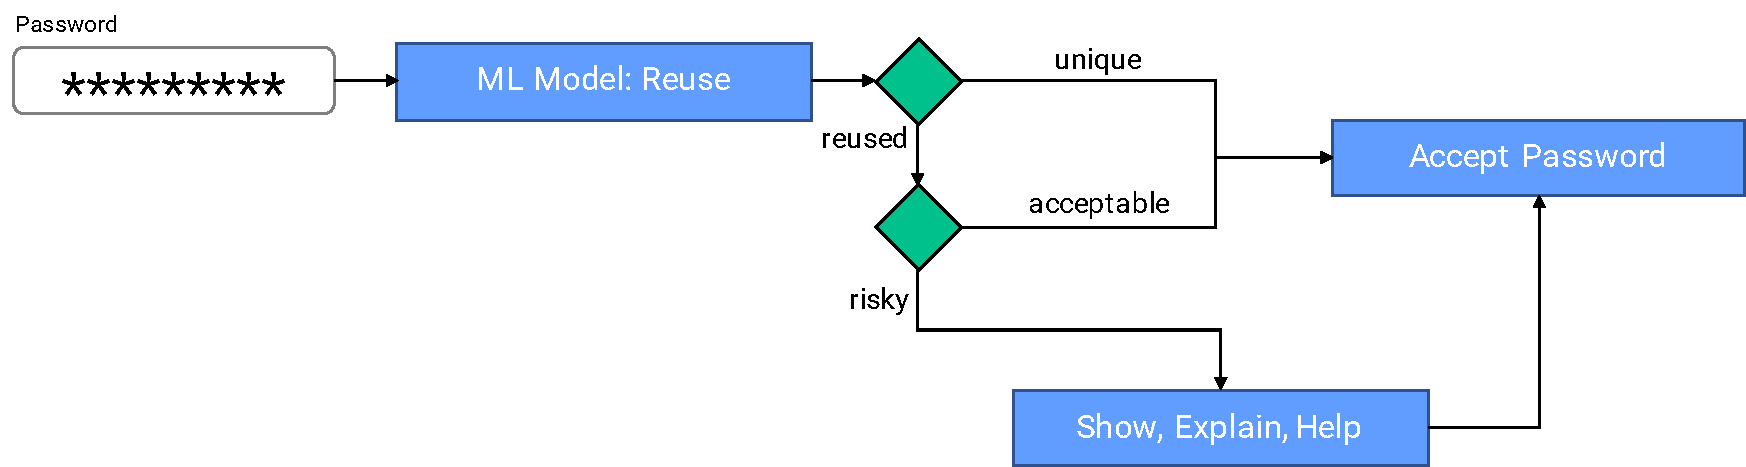
\includegraphics[width=\linewidth]{figures/summary/flow-chart}
	\caption{Personalized intervention for password reuse. The keystrokes inside a password field are analyzed by a machine learning model. If the password is unique, do not intervene. If the password is reused, but there are no signs for overlaps between categories, we can accept the password, too. However, if the password is reused across different categories, we use the show-explain-help paradigm to empower users to make an informed decision. In any case, the password is accepted to avoid being too restrictive. }
	\label{fig:summary:flow-chart}
\end{figure}

 
%Segreti \etal SOUPS 2017
%\cite{Seitz2017PersonalizingPasswordPolicies}
%\cite{Segreti2017AdaptivePolicies}

%\subsection{Keystrokes as Reuse Heuristics}
%Reuse is the worst. We should design a persuasive strategy that shows alternatives to reused passwords. As a first step, we need to detect that the password a user just entered has been reused on other websites. Since this is not bad per se, we also need to check how strong it is, and how likey it is a ``throw away'' password that users don't care about anyway. -- elaborate on this. Show an updated flow chart from CHI EA 


\subsection{Contextualizing Password Feedback}
Beyond personalization, which can be described as context-sensitive adaptation to the user, we should also consider tailoring password feedback to the system's context. For instance, we can create themed password meters to avoid habituation effects \cite{Ur2012HelpingUsersCreateBetterPasswords}. Kroeze and Olivier proposed using an evolving Pokemon as metaphor for the ``evolution state'' of the password \cite{Kroeze2012GamifyingAuthentication}. This kind of meter should probably be deployed on a game-related service, or directly for the registration page of Pokemon Go. As part of a design study, I created a themed password meter that matches the deployment context: Figure \ref{fig:summary:context-meter} shows a password meter that was originally created for a music-festival app. It is based on the \textit{share-explain-help} paradigm and is only one of many design options for this context. For instance, we could also choose a personalized social nudge and say ``\textit{only Justin Bieber fans use passwords like this}'' -- this could trigger in-/out-group biases and motivate some users to act differently. Optimally, such feedback systems are evaluated in situ, but to make it easier, we can use a cover story first, e.g. by creating a mock-website and recruit participants for usability tests thereof. Moreover, to assess the advantages of contextualized feedback, there should be a control group with neutral feedback.  

\begin{figure}
	\centering
	\begin{subfigure}[t]{\linewidth}
	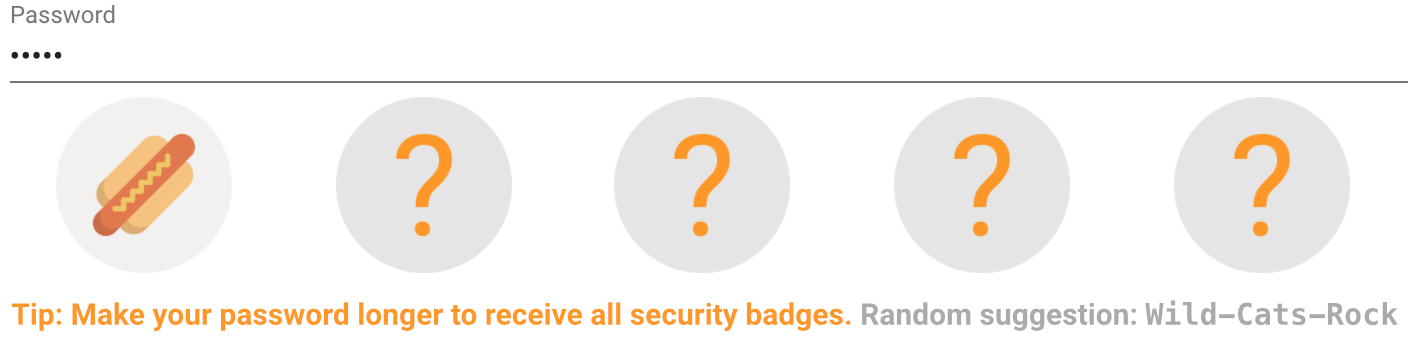
\includegraphics[width=\linewidth]{figures/summary/context-meter-01}
	\caption{\label{fig:summary:context-meter-01}Contextualized feedback and feedforward for a weak password.}
	\end{subfigure}
	\begin{subfigure}[t]{\linewidth}
	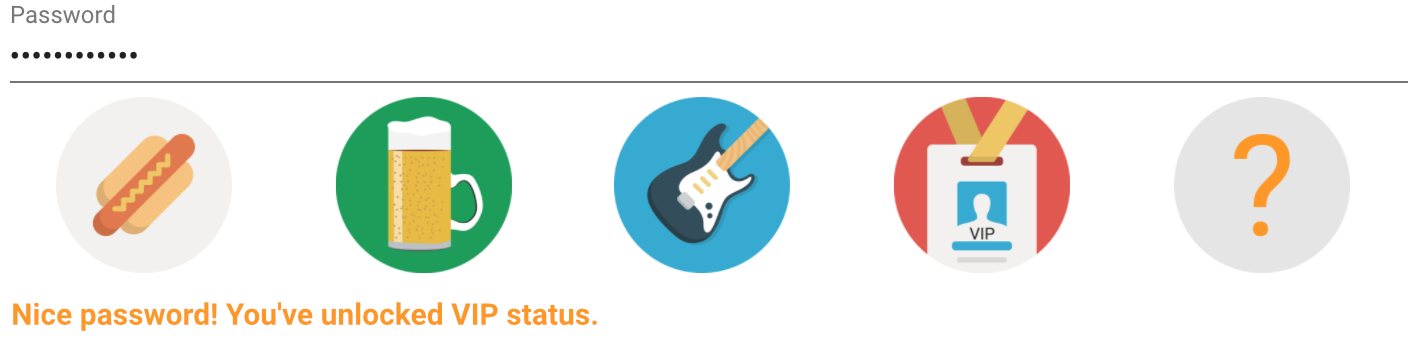
\includegraphics[width=\linewidth]{figures/summary/context-meter-04}
	\caption{\label{fig:summary:context-meter-04}When the password is sufficiently strong, provide reinforcing feedback.}
	\end{subfigure}
	\caption{\label{fig:summary:context-meter}A password meter for users of music festival app that uses context-related imagery to convey password strength. It is designed to drive curiosity. Feedback and feedforward follow the \textit{show-explain-help} paradigm.}
\end{figure}

%\subsection{What do other people do? Clichés and biased views of password selection strategies}
%people are biased to think that their password strategy is unique, i.e. they do not realize that other users behave similarly. it would be interesting to study the revelation process - ask people on the street how they think that others create their passwords for different categories. independent variables: who creates a password, for what context?
%
%social patterns helpful: Instead of saying a password is better than 90\% of other \textit{users} we could frame it as ``this password lowers your chance of being attacked by XX percent'' or ``this password is better than 90\% of passwords used on the internet''. issues: it's kind of hard to really be truthful here. deceptive in some ways and that's not something we want. 

\subsection{Solving Password Breach Aftermath}
% problem: password breaches every once in a while
Database breaches containing passwords occur frequently with different levels of severity depending on security standards at the affected service. 
% interesting problem: users cannot do anything about it but they are affected strongly.
Users face an immediate risk, but might be unaware of the situation, so they do not take swift measures to protect their account. 
% existing solutions: service providers invalidate accounts on their platforms, PWMs provide breach alarms. 
To mitigate this, service providers invalidate affected user accounts after breaches are detected. This is necessary to reestablish a secure overall system state where attackers cannot impersonate users on the platform. Usually, service providers inform users upon this countermeasure and prompt them to reset their passwords via email campaigns \cite{Huh2017TooBusy}. 
% existing solutions fall short because they fail to tell users which other accounts are affected (through reused credentials..)
While these countermeasures are unavoidable, they fall short of addressing the domino effect of reused passwords \cite{Ives2004DominoEffectReuse}. Many users do not understand the ramifications of a password breach and might only reset the password on the affected site. All other sites that share the same credentials remain at risk. 
% my idea: SPs should constantly monitor password leaks at third party websites to invalidate accounts that were affected on a third party.
I propose that service providers constantly monitor password leaks both on their own and on third party websites. In other words, while they might use a blacklist during account creation, there is usually no check-up mechanism that takes the updated risk-level into account. During this routine check-up, accounts that share credentials with affected third parties can be invalidated. The implementation should be straightforward with the aid of breach data freely available from different sources, e.g. \url{https://haveibeenpwned.com/Passwords}. 
%NIST's updated Electronic Authentication Guideline from August 2017 also includes a similar remark\footurl{https://pages.nist.gov/800-63-3/sp800-63b.html\#memsecretver}{29.03.2018}. 
% risks: users could be confused, emails may look like phising
However, there are a few issues that we need to solve in the future. First, freely available password lists rarely contain user-names to avoid targeted attacks. Second, if accounts are invalidated because a check-up has found a breached set of credentials, users might misunderstand the reasons for the account lock-down. Phishing attacks often use ``your account was locked down for security reasons'' as a hook to obtain users' real credentials. Sending out emails with reset prompts is thus especially dangerous because they may raise suspicion, and it is hard for novice users to verify if the prompt is legitimate.

Finally, it would be interesting to study how user behavior changes after a breach. So far, there have been attempts to collect initial data \cite{Huh2017TooBusy}, but there is far more that we have not measured, yet. For instance, it will be interesting to find out if personality traits are associated with user behavior after a breach. While it would be fair to assume that \textit{conscientious} users change their passwords more quickly and consistently, we did not necessarily see these behaviors in our own studies. Thus, there might be many opportunities for surprising insights.

\subsection{Re-locating Password Feedback} 
% final idea
% Password feedback in the wild can fail if people simply do not notice it:
A final problem to address in future work is the fact that many users simply do not \textit{notice} password feedback and therefore cannot re-assess their choice. 
% problem: most people look down on their hands when typing on regular desktop keyboards (not on mobile)
Many users look down on their hands when typing passwords on regular hardware keyboards, because they do have not mastered touch typing. During password entry, on-screen feedback is then out of sight. 
% interesting problem: it might explain why so many persuasive interventions do not unfold their full potential. 
This could explain why password meters have smaller impact on password selection in the wild: while study participants might take care to follow all on-screen instructions in an online experiment, users are often less focused on the screen in real-world tasks. 
% idea: relocate pw feedback closer to the hands.
Therefore, we study the impact of password feedback if it is relocated closer to the hands. 
% use touch bar to indicate feedback. 
The Touch Bar of current generations of the Apple MacBook Pro models is a visual output close to the hardware keys. It could be leveraged as display for both visual and textual password strength feedback \todo{craft a picture that visualizes the idea. take photo from hands at touchbar and trace the contours to make a mock-up}. To the best of my knowledge, this has not been investigated, but might be a feasible solution. 

%TODO maybe talk about mobile because we're in mobile first world. 

% risks: habituation (fewer variations possible)
% other situations that require relocation: on-screen keyboards might hide strength meters. figure

%\begin{figure}
%	\centering
%	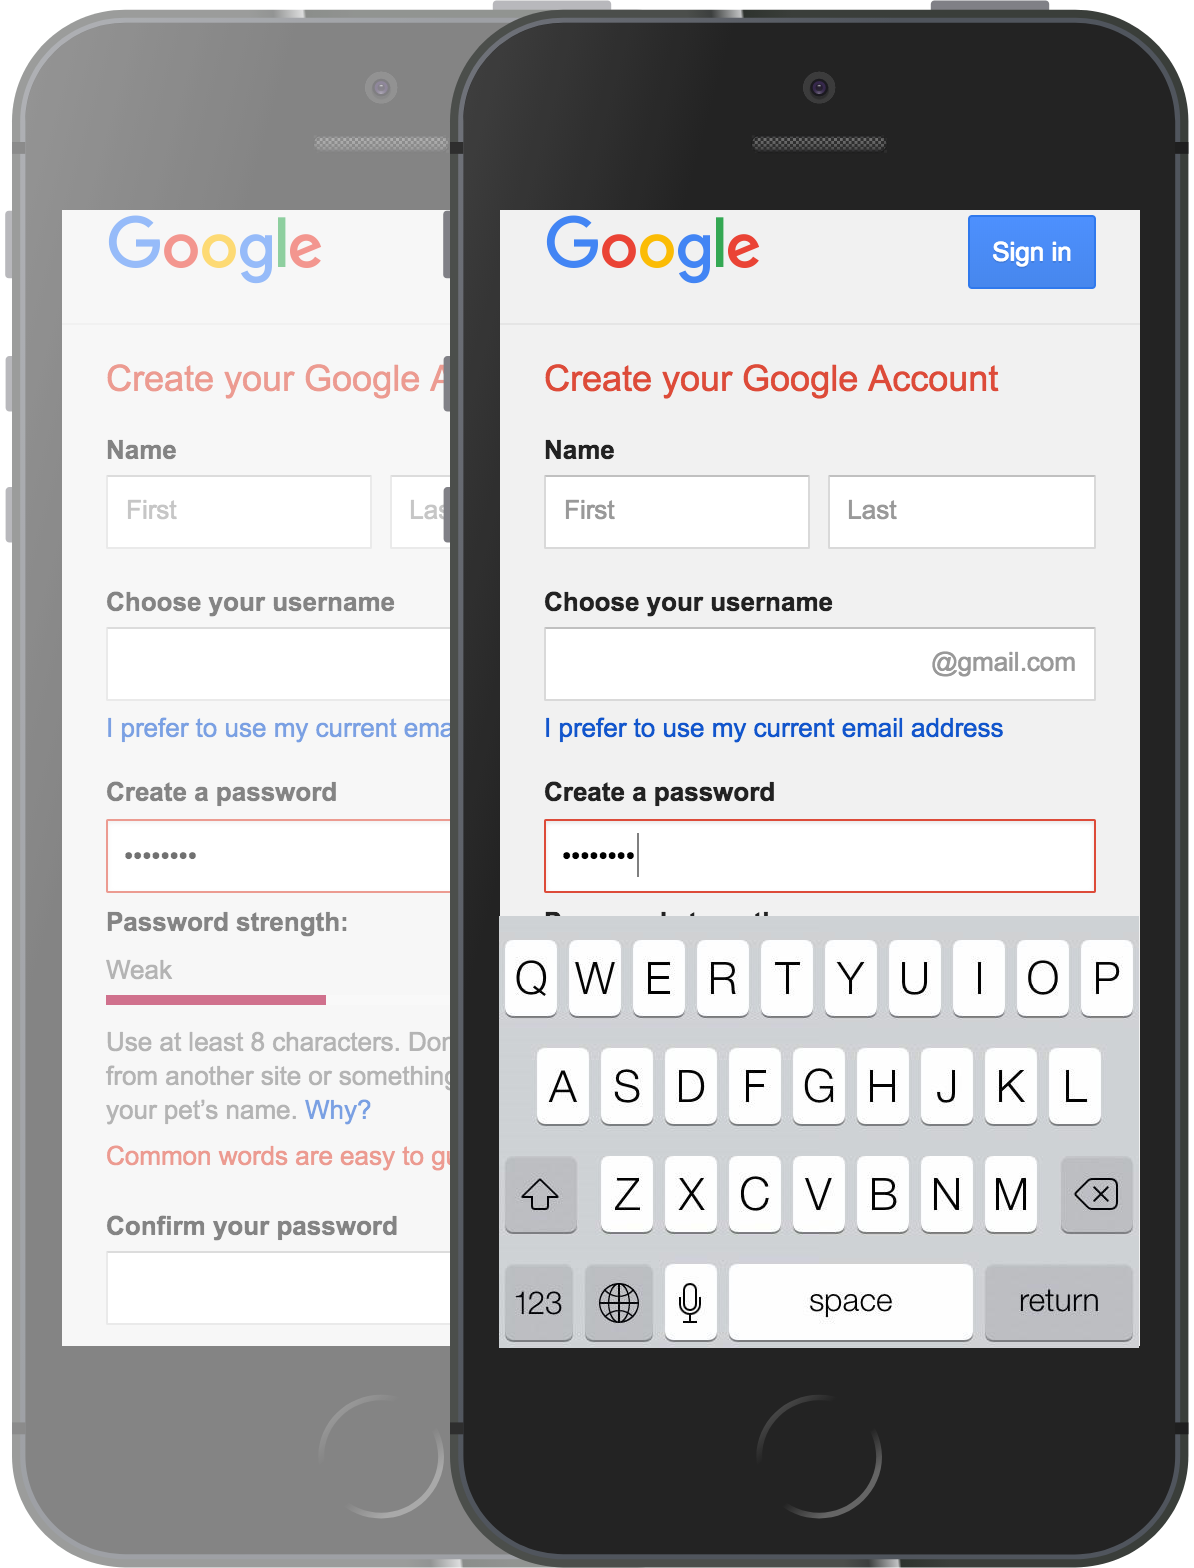
\includegraphics[width=0.5\linewidth]{figures/summary/osk-google-account}
%	\caption{\label{fig:osk-google-account} Password feedback is often hidden on mobiles while on-screen keyboards are open.}
%\end{figure}


\section{Final Thoughts}
%\begin{figure}[htpb]
%	\centering
%	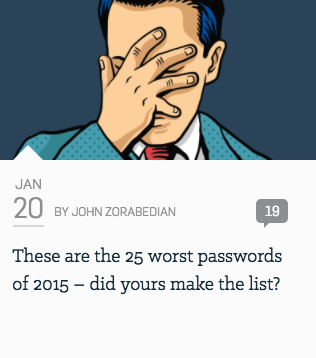
\includegraphics[width=0.3\linewidth]{shaming/nakedsecurity-sophos}
%	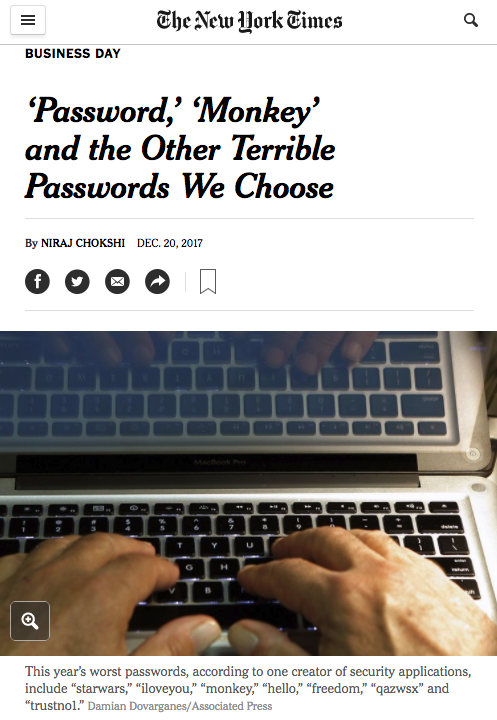
\includegraphics[width=0.3\linewidth]{shaming/nytimes}
%	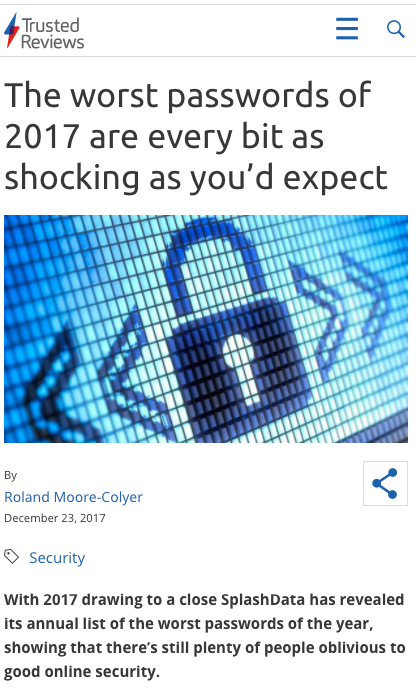
\includegraphics[width=0.3\linewidth]{shaming/trusted-reviews}
%	% i've got another screenshot from the register -- ironically there's no password meter on their site.
%\end{figure}
\begin{figure}
	\centering
	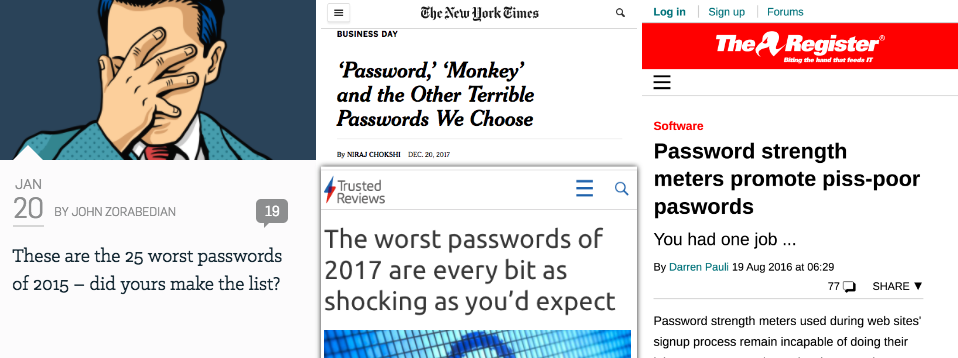
\includegraphics[width=\linewidth]{figures/summary/shaming-news}
	\caption{\label{fig:summary:shaming-news} The media are constantly shaming users for their ``bad passwords'', arguably as clickbait. However, this also acts as reinforcement because of the implicit normative message these headlines convey \cite{Cialdini2003CraftingNormativeMessages}. }
\end{figure}
I believe that users are not the weakest link in the authentication chain. There are always security mitigations on the system side that can take responsibility away from users. For instance, if all services had infinite resources to invest into penetration tests and alike, the need for exceptionally strong passwords vanishes. And although some user behavior is arguably risky, people should not be blamed for faulty systems that permit risks. Commentaries on the web and other media do the rest when they name and shame users for weak password behavior (see Figure \ref{fig:summary:shaming-news}). Perhaps, their intentions are good, but the subtext is different: Plenty of users are doing the same, so why would any one user act differently than the rest? This is maladroit framing of normative messages at best \cite{Cialdini2003CraftingNormativeMessages}.

% Future scenario
We have to face the truth: passwords annoy users. Most of us will not grief, if passwords become obsolete tomorrow. Probably, in the future, we will be able to make machines intelligent enough to independently decide whether a user should be granted access or not, all without explicit authentication. PCs and mobiles will automatically lock when the user is not in the vicinity. Natural interactions will enable us to tell virtual assistants to temporarily grant access to devices, e.g. by saying \textit{``Alexa, my daughter can use my iPad while we are driving to Italy, but make sure that she can only browse safe websites''}, all without the hassle of sharing PINs or enrolling biometric features. Naturally, a few drawbacks will remain, because perfect security cannot be guaranteed, and this will raise trust issues. People want to stay in charge and although passwords appear to be an inferior technology, they can achieve a higher level of perceived control. Thus, there will be not only a need but also a \textit{demand} for knowledge-based authentication in the future. Drawing on an analogy, passwords are perhaps the vinyl records in a world of ubiquitous music streaming: They are a bit clunky, impractical, and can be damaged through careless handling. On the other hand, experts still recommend them despite being an obsolete technology. People treasure them for years, often become collectors and try to find the rare, unique gems of long-lost quality. Once attacks on password alternatives like multimodal biometrics become commonplace, there might be a time when passwords see a revival like vinyl. 


%Apart from trust issues, users will then not need to worry about forgetting credentials or putting effort into creating strong passwords. 
% Passwords are bad. Let's hope passwords vanish at some point if passwords become obsolete tomorrow, many of us will not grief - and a few take-away messages from this thesis will be applicable to other authentication mechanisms too. Probably, in the nwe will be able to make machines intelligent enough to decide if a user should be granted access or not. But this also brings new problems.
% Maybe passwords are the vinyl records of usable security - everyone agrees that it's kind of an obsolete technology , they're a bit clunky, but there's something to them that ensures they don't disappear.



%\begin{itemize}
% \item  the media should stop shaming the users 
% \item  it's okay to forget passwords! reference to the article Franziska shared with me (SZ,  01.12.2017 ``Die Kunst zu vergessen'' \footurl{http://www.sueddeutsche.de/wissen/neurowissenschaft-die-kunst-zu-vergessen-1.3772438}{02.01.2018}.)
% \item 	ad networks for webpages can undermine any attempt to secure one's account. Too many websites show ads that can run harmful scripts. yes, adblockers do prevent this, but not everyone has one installed (especially novice users don't). Frightening research on this: \footurl{https://freedom-to-tinker.com/2017/12/27/no-boundaries-for-user-identities-web-trackers-exploit-browser-login-managers/}{02.01.2018}
%\end{itemize}
%
%It's interesting that often the same idea pops up every other year. so although there are no replication studies, evaluating the same idea multiple times with different setups and specifics, kind of goes in that direction. 

%TODO: take the ``pws are not going away'' section and put it here?


%TODO I have more thann 100 ``takeaways'' from papers. This could be a funny ``sermon'' too (Luther's 100 theses);


%%%%%%%%%%%%%%%%%%%%%%%%%%%%%%%%%%%%%%%%%%%%%%%%%%%%%%%%%%%%%%%%%%%%%%%%%%
%%%
%%% KICKED OUT
%%%
%%%
%%%%%%%%%%%%%%%%%%%%%%%%%%%%%%%%%%%%%%%%%%%%%%%%%%%%%%%%%%%%%%%%%%%%%%%%%%

% alternative: blacklist feature for password policy ``We are sorry, but this username-password combination appeared in a recent password leak at site XYZ''. 

%if a data leak is made public, sites can use the leaked passwords to audit the users on their sites. if they find that passwords have been compromised, they should decide (depending on a matching user name) if the password on their site should be invalidated and the user prompted to update it.
%
%kind of resembles a post-hoc blacklist.  
%
%catch: carefully craft Password Reset Emails \cite{Kim2017TooBusy}
%
%risks: users could be confused, looks like a phishing attack (why was my account hacked?)
%
%feature for password meters to determine stringency: 
%there could be a framework that uses \url{https://haveibeenpwned.com/API/v2} to adjust stringency 
%
%from \cite{Bishop1995ProactivePasswordChecking}: ``Many sites have responded to this threat with a reactive solution -- they scan their own password files and advise those users whose passwords they are able to crack. The problem with this solution is that while the local site is testing its security, the password file is still vulnerable from the outside. The other problems, of course, are that the testing is very time-consuming and only reports on those passwords it is able to crack. It does nothing to address user passwords which fall outside of the specific test cases (e.g., it is possible for a user to use as a password the letters ``query'' if this combination is not in the in-house test dictionary, it will not be detected, but there is nothing to stop an outside cracker from having a more sophisticated dictionary!).''

%\subsection{Helping to Make Sense of a Breach}
%how does user behavior change after a breach? not much says Huh \etal \cite{Huh2017TooBusy}. But it would be interesting to correlate other factors with altered behavior: do different personality traits influence how a user ``cleans up the mess'' after a breach?